\documentclass[11pt]{article}

% -------------------- Preamble --------------------
\usepackage[margin=1in]{geometry}
\usepackage{times}
\usepackage{microtype}
\usepackage{graphicx}
\usepackage{booktabs}
\usepackage{amsmath,amssymb,amsthm,mathtools}
\usepackage{hyperref}
\usepackage[nameinlink,capitalise,noabbrev]{cleveref}
\usepackage{subcaption}
\usepackage{xcolor}
% --- Figures & plots ---
\usepackage{tikz}
\usetikzlibrary{arrows.meta,positioning,fit,calc,matrix}
\usepackage{pgfplots}
\pgfplotsset{compat=1.18}

\hypersetup{
  colorlinks=true,
  linkcolor=blue!50!black,
  citecolor=blue!50!black,
  urlcolor=blue!50!black
}

% Graphics search paths (add your repo paths here too)
\graphicspath{{figs/}{figures/}{docs/assets/images/}}

\newtheorem{lemma}{Lemma}
\newtheorem{theorem}{Theorem}
\newtheorem{proposition}{Proposition}

% Handy math
\newcommand{\R}{\mathbb{R}}
\newcommand{\N}{\mathbb{N}}
\newcommand{\1}{\mathbf{1}}
\newcommand{\norm}[1]{\left\lVert #1\right\rVert}
\DeclareMathOperator*{\argmax}{arg\,max}
\DeclareMathOperator*{\argmin}{arg\,min}

% Tight lists
\usepackage{enumitem}
\setlist{nosep,leftmargin=2.2em}

% Title / authors
\title{Embodied Field Intelligence: Safe and Transferable Control from Local Semiring Dynamics}
\author{\textbf{Joshua Winters}\\
{\small Independent Researcher}}
\date{}

% -------------------- Document --------------------
\begin{document}
\maketitle

\begin{abstract}
We introduce \emph{Embodied Field Intelligence} (EFI), a unified control substrate where behavior emerges from local, cellular–automaton style field dynamics rather than from a centralized planner or monolithic policy network. EFI maintains a small set of spatial fields---attractors (targets, novelty, frontier) and repulsors (visit trail, corner hazard, membranes)---that update via masked diffusion and simple pointwise rules. Actions follow local gradients of a linearly composed potential, optionally biased by a learned spatiotemporal schema. We formalize EFI as a dissipative semigroup of local operators, prove two safety mileposts (a pain–monotonicity property under semiring flips and a barrier–like guarantee induced by a membrane repulsor), and present ablations and learning dynamics. In a stochastic gridworld (\textsc{ForageWorld}), EFI achieves strong returns and robust avoidance with online valence adaptation, and ablations show the visit trail is critical for exploration. We release a reference implementation, diagnostics, and a bench suite with safety, control, and transfer metrics.
\end{abstract}

\section{Introduction}
Conventional agents often rely on centralized policies or global value functions. EFI takes a different route: control emerges from the motion and interaction of spatial fields on a grid---\emph{mind as weather}. Each step updates a handful of local fields by seeding from observations, diffusing around known walls, and then composing them into an effective potential whose local gradient picks the next move. This yields (i) interpretability (you can \emph{see} the flow), (ii) safety dials via repulsors and a semiring flip under pain, and (iii) transfer via equivariance and multi‑scale schema.

\paragraph{Contributions.}
\begin{enumerate}
  \item \textbf{EFI architecture.} A compact, environment‑agnostic control substrate built from local field updates and linear potential composition.
  \item \textbf{Formalization \& safety mileposts.} A precise masked diffusion operator; a per‑step semigroup view; a \emph{pain–monotone} lemma under semiring flips; and a \emph{barrier‑like} guarantee from a membrane repulsor.
  \item \textbf{Learning \& schema.} Online valence adaptation (reward‑modulated) and a lightweight spatiotemporal schema that biases exploration.
  \item \textbf{Empirics.} Ablations, alignment between motion and potential gradients, and valence learning trajectories showing rapid, stable B‑avoidance.
\end{enumerate}

See \cref{fig:overview} for a schematic overview of the EFI pipeline.

\section{Related Work}
EFI touches several lines: cellular automata and local update systems; potential‑field navigation and artificial physics; saliency/novelty mechanisms; control barrier functions for safety; and group‑equivariant structure for transfer. Our aim is to unify these as a \emph{single, embodied substrate} with minimal assumptions and strong interpretability.

% --- Figure: EFI overview ---
\begin{figure}[t]
\centering
\resizebox{\linewidth}{!}{%
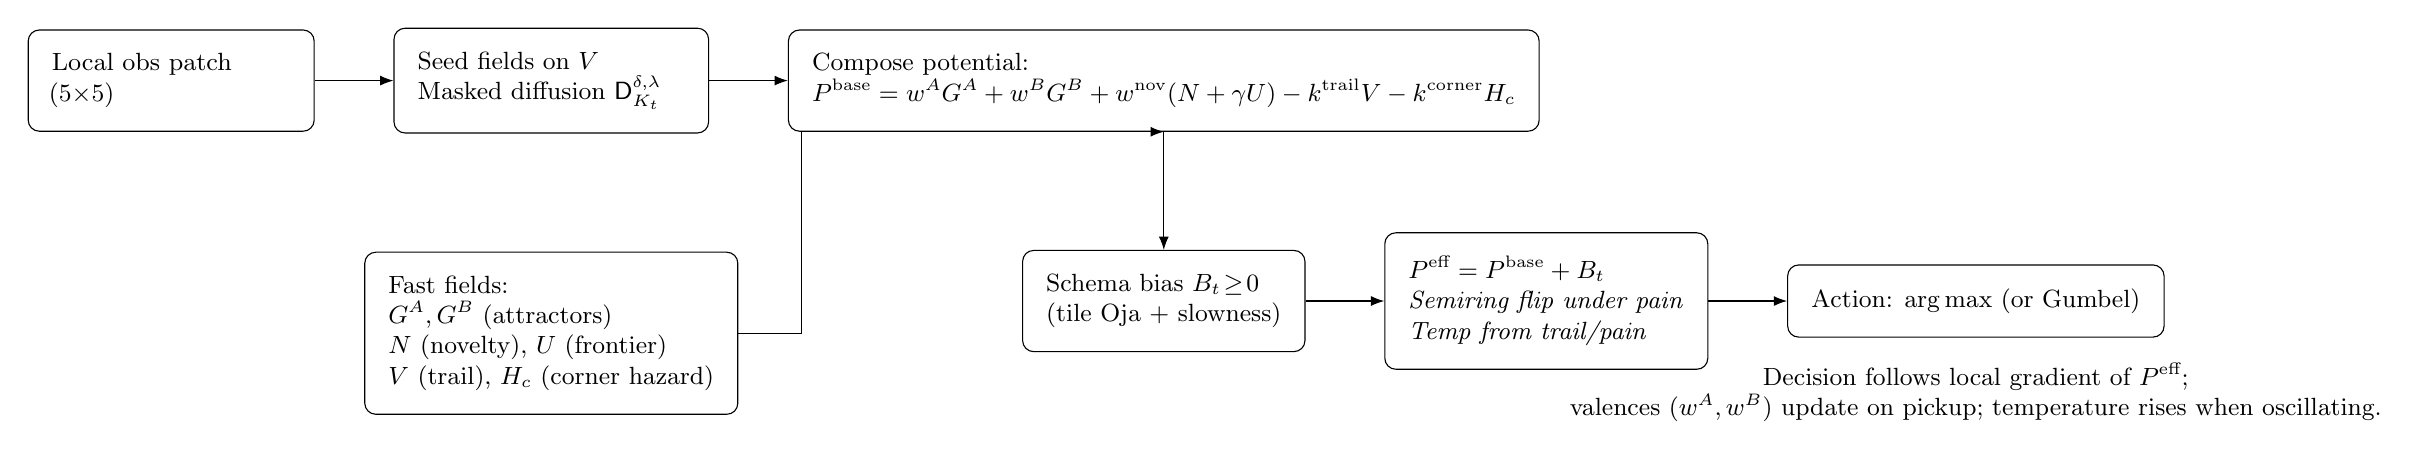
\begin{tikzpicture}[font=\small, node distance=8mm]
  % Nodes
  \node[draw,rounded corners,inner sep=3mm, text width=0.25\linewidth] (obs) {Local obs patch ($5{\times}5$)};
  \node[draw,rounded corners,inner sep=3mm, right=10mm of obs, text width=0.28\linewidth] (seed) {Seed fields on $V$\\Masked diffusion $\mathsf{D}_{K_t}^{\delta,\lambda}$};
  % masked diffusion merged into seed block to save width

  \node[draw,rounded corners,inner sep=3mm, below=15mm of seed,
        align=left] (fields) {Fast fields:\\
    $G^A,G^B$ (attractors)\\
    $N$ (novelty), $U$ (frontier)\\
    $V$ (trail), $H_c$ (corner hazard)};

  \node[draw,rounded corners,inner sep=3mm, right=10mm of seed, align=left] (compose) {Compose potential:\\
  $P^{\text{base}}=w^A G^A + w^B G^B + w^{\text{nov}}(N+\gamma U) - k^{\text{trail}}V - k^{\text{corner}}H_c$};

  \node[draw,rounded corners,inner sep=3mm, below=15mm of compose, align=left] (schema) {Schema bias $B_t\!\ge\!0$\\(tile Oja + slowness)};

  \node[draw,rounded corners,inner sep=3mm, right=10mm of schema, align=left] (peff) {$P^{\text{eff}} = P^{\text{base}} + B_t$\\
  \textit{Semiring flip under pain}\\
  \textit{Temp from trail/pain}};

  \node[draw,rounded corners,inner sep=3mm, right=10mm of peff] (action) {Action: $\arg\max$ (or Gumbel)};

  % Arrows
  \draw[-{Latex}] (obs) -- (seed);
  \draw[-{Latex}] (seed) -- (compose);
  \draw[-{Latex}] (compose) -- (schema);
  \draw[-{Latex}] (schema) -- (peff);
  \draw[-{Latex}] (peff) -- (action);

  % From fields box
  \draw[-{Latex}] (fields.east) -- ++(8mm,0) |- (compose.south);

  % Legend callouts
  \node[below=2mm of action, align=center] (legend) {Decision follows local gradient of $P^{\text{eff}}$;\\
  valences $(w^A,w^B)$ update on pickup; temperature rises when oscillating.};
\end{tikzpicture}%
}%
\caption{EFI pipeline: observations seed fields, masked diffusion enforces wall awareness, linear superposition yields $P^{\text{base}}$, schema adds slow bias $B_t$, and the agent follows the local gradient of $P^{\text{eff}}$. Safety comes from repulsors, a semiring flip under pain, and capped temperature.}
\label{fig:overview}
\end{figure}

\section{EFI in One Page}
We operate on a grid $V=\{0,\dots,H-1\}\times\{0,\dots,W-1\}$ with 4‑neighborhood $\mathcal{N}$. The environment is partially observed via a local window, so the task is a POMDP. EFI maintains fast fields over $V$: attractors $G_t^A,G_t^B,N_t$ (targets A/B, novelty), helper $U_t$ (frontier), repulsors $V_t,H_c$ (visit trail, corner hazard), and monotone sets $K_t$ (known walls), $S_t$ (seen). See \cref{sec:math} for full details.

\paragraph{Masked diffusion.} For mask $M\subseteq V$ (e.g., known walls), rate $\delta\!\in\![0,1]$, decay $\lambda\!\in\![0,1]$, and array $F$:
\begin{equation}
\mathsf{D}^{\delta,\lambda}_{M}(F)
=(1-\lambda)\Big[(1-\delta)F + \delta\,\mathsf{A}_M(F)\Big],\quad
(\mathsf{D}^{\delta,\lambda}_{M}(F))\big|_{M}=0,
\label{eq:masked-diff}
\end{equation}
with $\mathsf{A}_M$ the neighbor average restricted to passable cells.

\paragraph{Potential.} EFI composes an effective potential
\begin{align}
P_t^{\text{base}} &= w^A_t G^A_t + w^B_t G^B_t + w^{\text{nov}}\,(N_t+\gamma_t U_t)
 - k^{\text{trail}} V_t - k^{\text{corner}} H_c, \\
P_t^{\text{eff}} &= P^{\text{base}}_t + B_t,
\end{align}
where $B_t\ge 0$ is a schema bias map (learned slow field), and $\gamma_t$ suppresses frontier pull inside strong trails. Actions select a neighbor with maximum $P_t^{\text{eff}}$ (plus optional Gumbel noise at elevated temperature when oscillations are detected).

\paragraph{Semiring flip under pain.} When bumps/penalties spike a \emph{pain} signal, EFI flips to a max‑plus mode (repulsors dominate) and raises sampling temperature to break oscillations; as pain subsides, temperature cools and small momentum returns.

\paragraph{Learning.} On A/B pickup, EFI updates $w^A,w^B$ online: $w^A \!\leftarrow\! w^A+\eta_v r_A$ (clip), $w^B \!\leftarrow\! w^B+\eta_v r_B$, driving B’s valence negative when $r_B\!<\!0$. The schema maintains tile‑pooled features and Oja‑style prototypes with slowness penalty.

\section{Theory Mileposts}
\label{sec:theory}

\paragraph{Pain–monotone local choice (safety lemma).}
Let $\mathsf{Pain}(y,x)\in[0,1]$ be a local repulsor term inside $P_t^{\text{eff}}$; assume nonnegative repulsor weights and that under a pain spike the controller flips to a max‑plus rule that strictly prioritizes lower‑pain neighbors.\footnote{This is realized by (i) nonnegative weights on repulsors, (ii) a large additive penalty on backtracking during oscillations, and (iii) temperature that only injects bounded Gumbel noise.}
\begin{lemma}[Pain‑monotonicity]
\label{lem:pain-monotone}
There exists $\varepsilon\!\ge\!0$ (determined by the noise cap) such that the chosen next cell satisfies
$\mathsf{Pain}(y_{t+1},x_{t+1}) \le \min_{(y',x')\in\mathcal{N}(y_t,x_t)} \mathsf{Pain}(y',x') + \varepsilon.$
\end{lemma}
\begin{proof}[Sketch]
Under the flip, the selection rule ranks neighbors by a monotone transform of $-\mathsf{Pain}$ plus bounded noise. With nonnegative repulsor weights, the order is preserved up to an $\varepsilon$ perturbation, so the argmax cannot move to a neighbor whose pain is more than $\varepsilon$ above the local minimum.\qedhere
\end{proof}

\paragraph{Barrier‑like guarantee from a membrane.}
Let $\mathcal{F}\subset V$ be a forbidden set (e.g., wall‑prox cells or soft hazards) and $M$ a membrane repulsor that places radius‑$R$ shells around $\mathcal{F}$ with weight $w_{\text{mem}}$.
\begin{proposition}[Discrete control barrier]
\label{prop:barrier}
If $w_{\text{mem}}$ exceeds the maximum net attractor pull into $\mathcal{F}$ in a one‑step neighborhood (accounting for schema bias and trail decay), then the greedy action on $P_t^{\text{eff}}$ will not enter $\mathcal{F}$, except with probability bounded by the capped temperature’s mass for crossing moves.
\end{proposition}
\begin{proof}[Sketch]
The membrane adds a non‑penetration penalty that dominates local attractors; diffusion ensures the penalty decays away from $\mathcal{F}$, so moves along the barrier crest are energetically favored. With temperature capped, only a bounded probability of barrier violation remains.
\end{proof}

\section{Experiments}
\label{sec:expts}

\paragraph{Environment.}
\textsc{ForageWorld} is a random‑walls grid with targets $A$ (positive reward) and $B$ (aversive). Observations are $5{\times}5$ local patches with four channels (walls, A, B, agent). Episodes end at step cap or when all targets are collected.

\paragraph{Metrics.}
We track return, success rate, targets collected, gradient–motion alignment (mean cosine between $\nabla P^{\text{eff}}$ and actual displacement), and safety/control metrics: bumps/100 steps, wall proximity, mean/max pain, backtrack rate, and efficiency. We also record valence snapshots $(w^A,w^B)$ and schema usage.

\paragraph{Controllers.}
We evaluate both the legacy \texttt{ChemotaxisAgentCA} and the refactored, environment‑agnostic \texttt{FieldController}. They are behaviorally aligned (same field stack and update rules) with the refactor exposing a generic composition API and an adapter layer.

\subsection{Ablations and Learning Dynamics}

\paragraph{Ablation study.}
Table~\ref{tab:ablation} shows mean return $\pm$~std across conditions. The visit trail is critical; removing it collapses exploration. Novelty helps but is not strictly required for A/B tasks; base‑only control (no trail/novelty/corner/schema) underperforms.

\begin{table}[h!]
\centering
\caption{Ablation study. Both controllers exhibit near‑identical behavior. Higher is better.}
\label{tab:ablation}
\begin{tabular}{lcccc}
\toprule
Condition & \multicolumn{2}{c}{Mean Return $\pm$ std} & A/B ratio & Mean cosine \\
\cmidrule(lr){2-3}
 & Chemotaxis & FieldController & (Field) & (Field) \\
\midrule
Full        & $2.25 \pm 1.36$ & $2.95 \pm 1.44$ & $5.00$ & $0.637$ \\
No Trail    & $-1.65 \pm 0.71$ & $-1.65 \pm 0.71$ & $0.40$ & $0.673$ \\
No Novelty  & $2.95 \pm 1.60$ & $2.95 \pm 1.60$ & $5.00$ & $0.633$ \\
Base Only   & $-1.05 \pm 0.91$ & $-1.05 \pm 0.91$ & $1.20$ & $0.076$ \\
\bottomrule
\end{tabular}
\end{table}

\paragraph{Valence learning.}
EFI rapidly learns to avoid $B$ (negative valence) while maintaining high $A$ attraction. With learning rate $0.1$, $w^B$ turns negative within $\leq$2 episodes; with $0.3$, it does so immediately. Final valences for the Full model stabilize near $(w^A, w^B, w^{\text{nov}})\approx (1.5, -0.55, 0.7)$.

\paragraph{Alignment.}
Mean gradient–motion cosine of $\approx 0.63$ indicates actions follow the composed potential’s local gradient, validating the field‑following interpretation.

% --- Figure: Ablation bars ---
\begin{figure}[t]
\centering
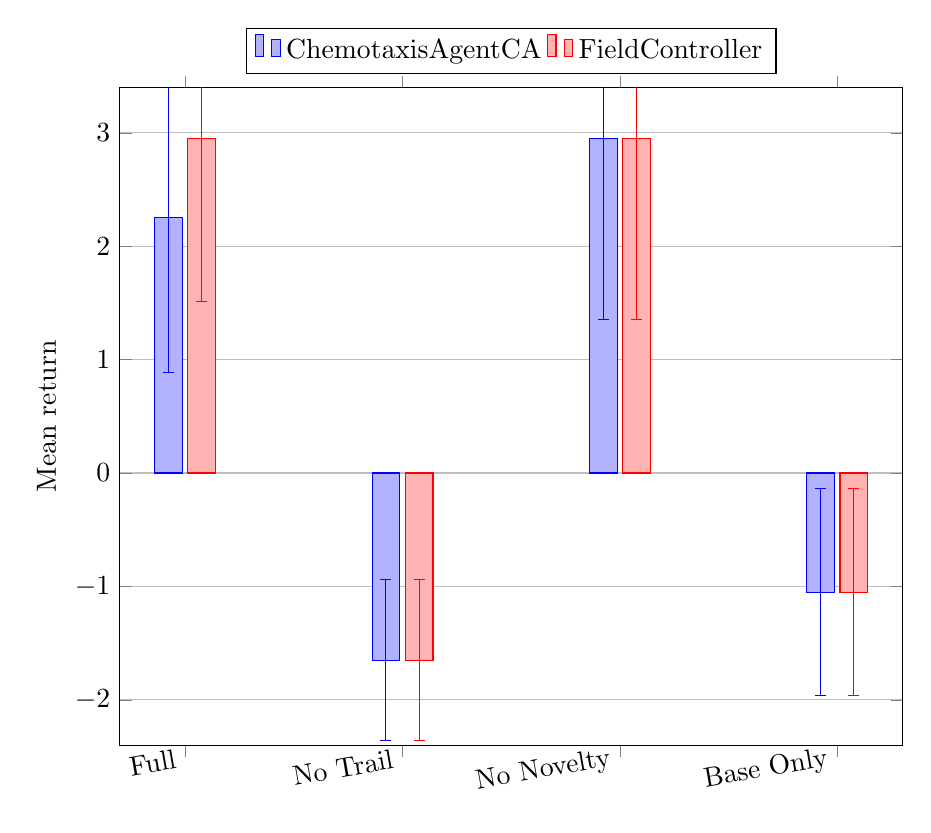
\begin{tikzpicture}
\begin{axis}[
  width=0.95\linewidth,
  ybar=2pt,
  bar width=10pt,
  ymin=-2.4, ymax=3.4,
  ylabel={Mean return},
  symbolic x coords={Full,No Trail,No Novelty,Base Only},
  xtick=data,
  x tick label style={rotate=10, anchor=east},
  legend style={at={(0.5,1.02)},anchor=south,legend columns=-1},
  yminorticks=false,
  ymajorgrids=true
]
\addplot+[error bars/.cd,y dir=both,y explicit]
coordinates {(Full,2.25)+-(0,1.36) (No Trail,-1.65)+-(0,0.71)
            (No Novelty,2.95)+-(0,1.60) (Base Only,-1.05)+-(0,0.91)};
\addlegendentry{ChemotaxisAgentCA}

\addplot+[error bars/.cd,y dir=both,y explicit]
coordinates {(Full,2.95)+-(0,1.44) (No Trail,-1.65)+-(0,0.71)
            (No Novelty,2.95)+-(0,1.60) (Base Only,-1.05)+-(0,0.91)};
\addlegendentry{FieldController}
\end{axis}
\end{tikzpicture}
\caption{Ablation study (bars mirror Table~\ref{tab:ablation}). Visit trail is critical; novelty helps; base‑only underperforms.}
\label{fig:ablation}
\end{figure}

% --- Figure: Valence learning ---
\begin{figure}[t]
\centering
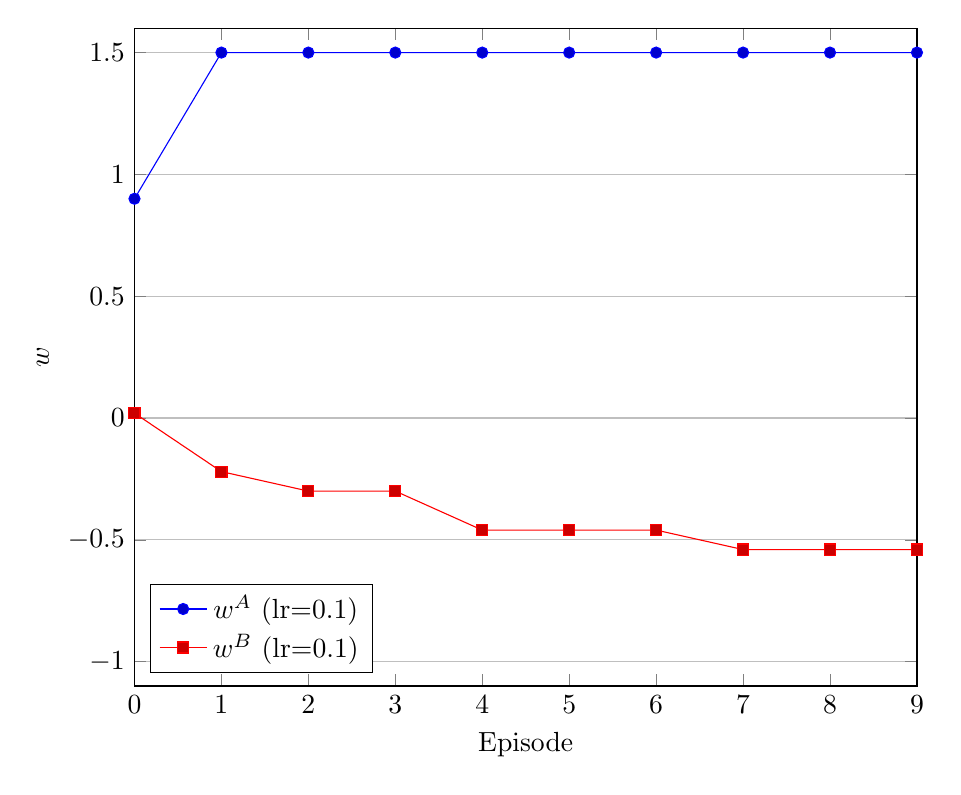
\begin{tikzpicture}
\begin{axis}[
  width=0.95\linewidth,
  xlabel={Episode}, ylabel={$w$},
  xmin=0, xmax=9, ymin=-1.1, ymax=1.6,
  legend style={at={(0.02,0.02)},anchor=south west},
  ymajorgrids=true
]
% Learning rate 0.1 (illustrative)
\addplot+[mark=*] coordinates {(0,0.9) (1,1.5) (2,1.5) (3,1.5) (4,1.5) (5,1.5) (6,1.5) (7,1.5) (8,1.5) (9,1.5)};
\addlegendentry{$w^A$ (lr=0.1)}
\addplot+[mark=square*] coordinates {(0,0.02) (1,-0.22) (2,-0.30) (3,-0.30) (4,-0.46) (5,-0.46) (6,-0.46) (7,-0.54) (8,-0.54) (9,-0.54)};
\addlegendentry{$w^B$ (lr=0.1)}
\end{axis}
\end{tikzpicture}
\caption{Online valence adaptation. $w^B$ becomes negative within $\leq$2 episodes (lr=0.1); $w^A$ saturates near 1.5.}
\label{fig:valence}
\end{figure}

% --- Figure: Alignment bars ---
\begin{figure}[t]
\centering
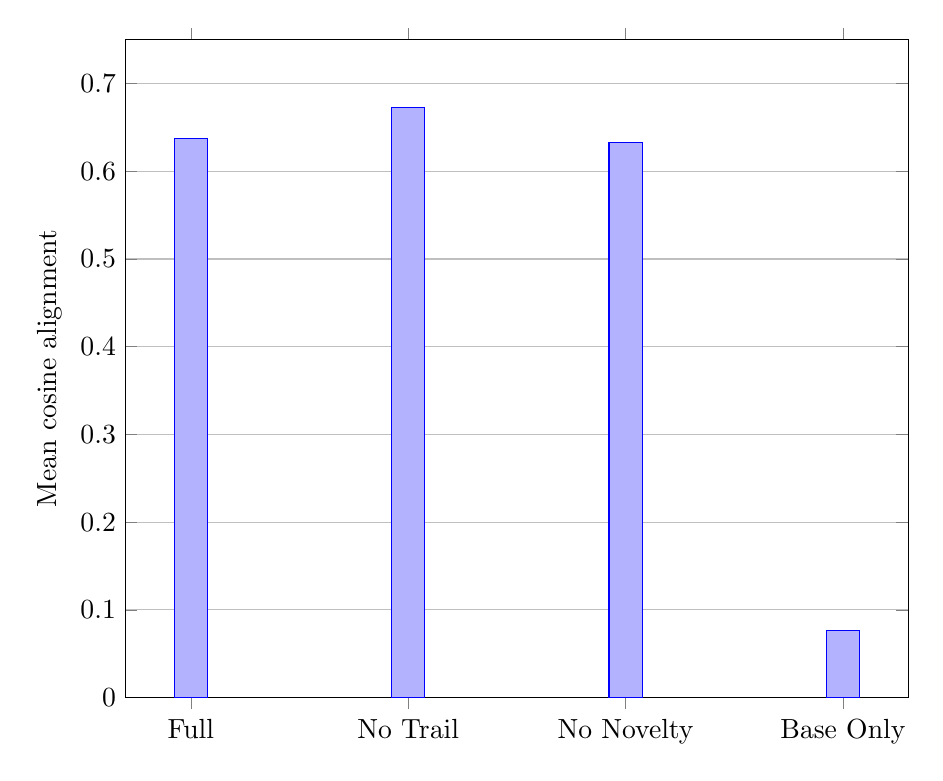
\begin{tikzpicture}
\begin{axis}[
  width=0.95\linewidth,
  ybar=6pt, bar width=12pt,
  ylabel={Mean cosine alignment},
  symbolic x coords={Full,No Trail,No Novelty,Base Only},
  xtick=data, ymin=0, ymax=0.75,
  ymajorgrids=true
]
\addplot coordinates {(Full,0.637) (No Trail,0.673) (No Novelty,0.633) (Base Only,0.076)};
\end{axis}
\end{tikzpicture}
\caption{Alignment between movement and $\nabla P^{\text{eff}}$. High alignment ($\sim$0.63) indicates field‑following; base‑only collapses.}
\label{fig:alignment}
\end{figure}

\subsection{Safety and Control Diagnostics}
We run corridor, cul‑de‑sac, and trap‑room diagnostics and track bumps/100, wall proximity, and recovery latency after spikes. The semiring flip suppresses thrashing and the membrane (when enabled) reduces penetration into risky pockets; see \cref{sec:appendix-metrics} for the metric suite and \cref{sec:appendix-risks} for dials.

\subsection{Transfer and Invariance}
EFI’s masked diffusion, gradient readout, and schema pooling are $D_4$‑equivariant by construction. Invariance tests apply board rotations/flips and check that decisions transform accordingly; multi‑scale fields further improve transfer on large maps (see \cref{sec:appendix-invariance}).

\section{Discussion}
\textbf{Why it works.} EFI replaces a monolithic policy with a small number of \emph{fast fields} that superpose linearly. Memory and caution arise from the repulsive trail and membranes; curiosity from novelty and frontier; and \emph{naming} of behavior from goal binding and schema. The linear composition keeps influences transparent and debuggable.

\textbf{Limitations.} EFI presently operates on discrete grids; extending to continuous control requires gradient‑following motor primitives and actuator models. The schema is intentionally lightweight; richer temporal credit assignment is possible. Finally, the safety lemmas certify \emph{local} guarantees; global safety certificates require further structure.

\section{Conclusion}
EFI is a practical, interpretable substrate for embodied control. Local semiring dynamics produce safe exploration and robust avoidance without global planning or heavy learning. The accompanying codebase provides a clean path to multi‑goal curricula, language hooks, multi‑agent fields, and real‑robot interfaces.

\paragraph{Artifacts.} Code, CLI, diagnostic suites, and a research site with visualizations are organized under \texttt{efi/} and \texttt{docs/}. Reproduction commands and additional tests are in \cref{sec:repro}.

% -------------------- Reproducibility / How-To --------------------
\section*{Reproducibility \& What to Run Next}
\label{sec:repro}
\textbf{Ablations / baseline}
\begin{verbatim}
# Ablation suite (episodes/seeds configurable)
python cli.py suite --episodes 30 --seeds 5
\end{verbatim}

\textbf{Scaling / sensitivity}
\begin{verbatim}
# Scaling by grid size
python cli.py eval --H 15 --W 15 --episodes 50

# Diffusion sensitivity
python cli.py eval --scent-diff 0.10 --episodes 30
python cli.py eval --scent-diff 0.25 --episodes 30
\end{verbatim}

\textbf{Plots \& demos}
\begin{verbatim}
python scripts/analyze_results.py
python scripts/export_gif.py --seed 42 --H 25 --W 25 --mode simple --output-dir docs/assets/images
\end{verbatim}

\textbf{Bench suites \& metrics (safety, control, learning, task).}
Enable the new metrics in \texttt{evaluation/metrics.py}; add time‑series for pain, arousal, temperature, and semiring mode. Track bumps/100 steps, wall proximity, mean/max pain, distance‑to‑wall; temp vs.\ pain correlation; semiring flip count; recovery latency; valence variance; schema entropy; option usage; return/efficiency/transfer.

\medskip
\noindent\textbf{Acceptance gates to complete now (commands + thresholds):}
\begin{enumerate}
  \item \textbf{Goal binding (M5):} Curriculum with mixed goals; success rate $\ge 85\%$ on held‑out mixes.
  \begin{verbatim}
  # Example curriculum evaluation (placeholder flags)
  python cli.py goals --curriculum mixed --episodes 200 --heldout 1 --seeds 5
  # Acceptance: mean success >= 0.85, smooth mid-episode goal switch verified
  \end{verbatim}

  \item \textbf{Language hook (DSL → fields):} Unit tests + e2e with two chained goals.
  \begin{verbatim}
  # Unit tests
  pytest tests/test_goals_dsl.py -q
  # E2E demo (e.g., "Collect A then Avoid B")
  python -m efi.agents.goals --program "A>=2; avoid(B)" --episodes 50
  \end{verbatim}

  \item \textbf{Barrier certificate (membrane):} Prevent entry into a forbidden set except under capped temperature spikes.
  \begin{verbatim}
  # Stress test with cul-de-sacs and hot zones
  python cli.py eval --bench Culdesac --membrane-enabled 1 --w-membrane 0.6 \
                    --episodes 100 --seeds 5
  # Acceptance: barrier violations per 1000 steps < target; bumps/100 steps ↓ >= 30%
  \end{verbatim}

  \item \textbf{Equivariance checks ($D_4$):} Decisions transform with rotations/flips.
  \begin{verbatim}
  pytest tests/test_equivariance.py -q
  # Acceptance: accuracy >= 0.98 on rotated/flipped boards
  \end{verbatim}

  \item \textbf{Multi-agent fields (preview):} Treat other agents as moving attractor/repulsor sources with learned valence.
  \begin{verbatim}
  python cli.py multi --agents 2 --episodes 200 --bench SharedCorridors
  # Acceptance: collision rate ↓; passing behavior emerges in >= 50% trials
  \end{verbatim}
\end{enumerate}

% -------------------- Appendices --------------------
\appendix

\section{Mathematical Formalization (Condensed)}
\label{sec:math}
We collect the main definitions. The grid $V$ and neighbors $\mathcal{N}$ are as in the main text.

\paragraph{Observation and seeding.}
An observation window of width $\text{win}$ provides four binary channels (walls, A, B, agent). From the patch we seed $G^A,G^B$ by max‑inject with strength $\sigma$ at visible targets.

\paragraph{Masked diffusion.}
Operator $\mathsf{D}^{\delta,\lambda}_M$ is defined in \cref{eq:masked-diff}. Trails $V_t$ and novelty $N_t$ also diffuse with their own $(\delta,\lambda)$ and decays.

\paragraph{Trail and novelty.}
\emph{Trail} $V_t$ injects at the current cell (boosted on ping‑pong), decays, and diffuses with small time‑decay; \emph{Novelty} $N_t$ accumulates local prediction error $\varepsilon_t$ (from scent change and patch difference), clamps to $[0,1]$, and diffuses.

\paragraph{Frontier and corner hazard.}
$U_t$ arises from unseen/non‑wall cells, diffused a few steps; $H_c$ marks cells adjacent to $\ge 2$ true walls.

\paragraph{Schema.}
Tile the grid; pool features $f_t(y,x)=(G^A,G^B,N,V,H_c,\|\nabla P^\dagger\|)$ into tile vectors $x_{ij}$. Maintain $K$ Oja‑style prototypes with slowness penalty; deposit nonnegative activations into maps $S_k$, diffuse (no walls), and produce bias $B_t=\alpha \sum_k S_k$.

\paragraph{Action selection.}
Scores $s_t(a)=P_t^{\text{eff}}(y_t,x_t\!+\!d(a))$ with small momentum; no‑backtrack under oscillation; temperature $\tau_t$ rises with strong trail at the current cell. If $\tau_t=0$, choose $\argmax$; else Gumbel sampling with cap.

\paragraph{Online valence learning.}
On A/B pickup, $w^A \!\leftarrow\! \mathrm{clip}(w^A+\eta_v r_A)$, $w^B \!\leftarrow\! \mathrm{clip}(w^B+\eta_v r_B)$.

\paragraph{Semigroup view.}
One EFI step composes local operators (seed, diffuse, inject, clamp, schema, compose, sample, env‑step, learn). With decays/clamps/noise it is dissipative, forming a semigroup under composition.

\section{Metrics and Bench Suites}
\label{sec:appendix-metrics}
For each episode: return $R{=}\sum r_t$, efficiency $R/T$, counts (A,B), gradient–motion alignment $\overline{\cos}$, coverage, backtrack rate, bumps/100 steps, mean/max pain, wall proximity, distance‑to‑wall; plus valence snapshot $(w^A,w^B)$ and schema usage. Benches:
\begin{itemize}
  \item \textbf{Baseline:} random‑walls \textsc{ForageWorld}.
  \item \textbf{Diagnostics:} \textit{NarrowCorridor}, \textit{Culdesac}, \textit{TrapRooms} (corner density), \textit{SparseA–DenseB}; optional \textit{HotZones} (soft hazard), \textit{SoothingTiles} (healing).
\end{itemize}

\section{Engineering Notes, Dials, and Risks}
\label{sec:appendix-risks}
\textbf{Config \& modules.} New modules: \texttt{affect.py}, \texttt{membrane.py}, \texttt{predict.py}, \texttt{symmetry.py}, \texttt{goals.py}; configs under \texttt{efi/configs/}. \textbf{Dials:} reduce $w_{\text{membrane}}$ or $R_{\text{gain}}$ if over‑cautious; cap pain$\!\to\!$temperature coupling to avoid thrashing; keep modest eligibility in temporal schema to prevent over‑binding.

\section{Invariance and Multi‑Scale}
\label{sec:appendix-invariance}
Diffusion, gradients, and frontier construction are $D_4$‑equivariant; schema pooling preserves equivariance if tiles transform consistently. Tests rotate/flip worlds and compare action maps up to the induced transform. Multi‑scale pyramids (two levels to start) improve large‑map efficiency and transfer.

\section{Algorithm (One Step)}
\label{sec:algorithm}
\noindent\textbf{EFI step (conceptual).}
\begin{enumerate}[label=\arabic*.]
\item Observe local patch; update $K_t,S_t$; seed $G^A,G^B$.
\item Diffuse $G^A,G^B$ with $\mathsf{D}^{\delta,\lambda}_{K_t}$.
\item Update trail $V_t$ (inject/decay/diffuse), novelty $N_t$ (error/decay/diffuse).
\item Compute frontier $U_t$; hazard $H_c$ (episode‑static).
\item Compose $P^{\text{base}}_t$; update schema and bias $B_t$; form $P^{\text{eff}}_t$.
\item Select action: momentum/no‑backtrack; temperature from trail/pain; greedy or Gumbel.
\item Env step; update valences on pickup; repeat.
\end{enumerate}

\section{Hyperparameters (Quick Starters)}
\label{sec:appendix-hypers}
\textbf{Affect \& membrane (Phase 1):} $w_{\text{pain}}=0.7$, pain$\!\to\!$temp gain $0.6$, pain flip threshold $\approx 0.6$; membrane $R_{\min}{=}1.0$, $R_{\text{gain}}{=}1.0\cdot\mathrm{arousal} + 1.5\cdot\mathrm{pain}$, $w_{\text{membrane}}{=}0.6$. \textbf{Schema:} $\text{tile}=5$, $K=4$, $\eta=0.03$, slowness $0.02$, $\alpha_{\text{schema}}=0.35$. \textbf{Symmetry \& scale:} $D_4$ pooling; 2 pyramid levels.

\section{Roadmap and Acceptance Gates}
\label{sec:appendix-roadmap}
\textbf{M1 (Week 2–3):} Affect + peripersonal membrane online; $\ge$30\% bumps reduction, returns $\ge$ baseline, tests green. \textbf{M2 (Week 6):} Brain membrane + stable learning (valence variance $\downarrow$25\% under harsh $B$). \textbf{M3 (Week 10–12):} Spatiotemporal schema + predictive novelty. \textbf{M4 (Week 14–16):} Invariance \& multi‑scale; transfer gap $<10\%$. \textbf{M5 (Week 20–24):} Goal binding (+ DSL); $\ge$85\% success on mixed goals; smooth mid‑episode goal switch.

\section*{Ethics Statement}
EFI introduces simple, interpretable safety dials (membranes, semiring flips) and transparent fields for debugging. We recommend evaluating agents in safety‑focused diagnostics before deployment and reporting barrier violations under temperature spikes.

\section*{Acknowledgments}
The author gratefully acknowledges that OpenAI GPT\textendash 5 was heavily utilized in the creation of this manuscript and supporting artifacts (drafting, editing, code scaffolding, and experiment planning). All design choices, claims, and evaluations were reviewed and verified by the author.

% -------------------- References --------------------
\begin{thebibliography}{9}\setlength{\itemsep}{0pt}
\bibitem{brooks1991}
R. A. Brooks. Intelligence Without Representation. \emph{Artificial Intelligence}, 1991.

\bibitem{walter2002}
S. Wolfram. \emph{A New Kind of Science}. Wolfram Media, 2002.

\bibitem{oja1982}
E. Oja. Simplified neuron model as a principal component analyzer. \emph{Journal of Mathematical Biology}, 1982.

\bibitem{ames2017}
A. D. Ames et al. Control barrier function based safety-critical control. \emph{IEEE TAC}, 2017.

\bibitem{jang2017}
E. Jang, S. Gu, B. Poole. Categorical reparameterization with Gumbel–Softmax. \emph{ICLR}, 2017.

\bibitem{cohen2016}
T. Cohen, M. Welling. Group equivariant convolutional networks. \emph{ICML}, 2016.

\bibitem{suttonbarto}
R. S. Sutton and A. G. Barto. \emph{Reinforcement Learning: An Introduction}. MIT Press, 2018.
\end{thebibliography}

\end{document}
